\documentclass[tikz,border=12pt]{standalone}
\usepackage{amsmath,amssymb}
\usetikzlibrary{calc,arrows.meta}

\begin{document}
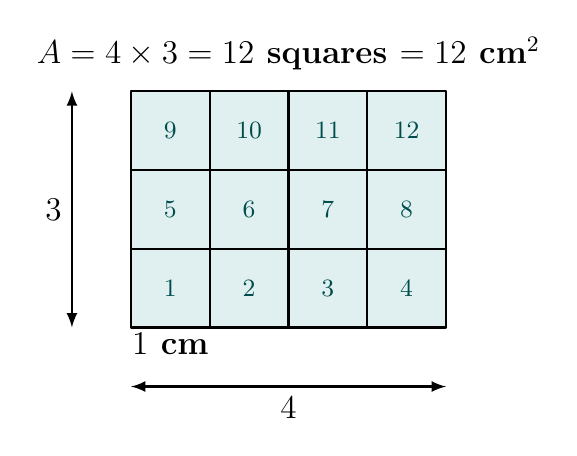
\begin{tikzpicture}[>=latex, line cap=round, line join=round]

  % Count unit squares and fill the grid 4 by 3
  \foreach \x in {0,...,3}{
    \foreach \y in {0,...,2}{
      \draw[thick, fill=teal!12] (\x,\y) rectangle (\x+1,\y+1);
    }
  }
  % number the squares 1..12 lightly
  \foreach \y/\base in {0/0, 1/4, 2/8}{
    \foreach \x in {0,...,3}{
      \node[font=\small\color{teal!60!black}] at
        ({\x+0.5},{\y+0.5}) {\pgfmathtruncatemacro{\n}{\base+\x+1}\n};
    }
  }

  % unit marker on one grid square edge
  \node[font=\large\bfseries, below] at (0.5,0.05) {$1$ cm};

  % dimension arrows
  \draw[thick, <->] (0,-0.75) -- (4,-0.75)
    node[midway, below, font=\large\bfseries] {$4$};
  \draw[thick, <->] (-0.75,0) -- (-0.75,3)
    node[midway, left, font=\large\bfseries] {$3$};

  % conclusion label
  \node[font=\large\bfseries, above] at (2,3.15)
    {$A = 4 \times 3 = 12$ squares $= 12$ cm$^2$};

\end{tikzpicture}
\end{document}
